% this is the one from github LLLL
\section{\label{sec:AnatRationale}Anatomical Rationale}

%%%%%%%%%%%%%%%%%%%%%%%%%%%%%%
%Figure 1 (Beatriz and Humin)
%%%%%%%%%%%%%%%%%%%%%%%%%%%%%%

\begin{figure}[ht]
  \centering
  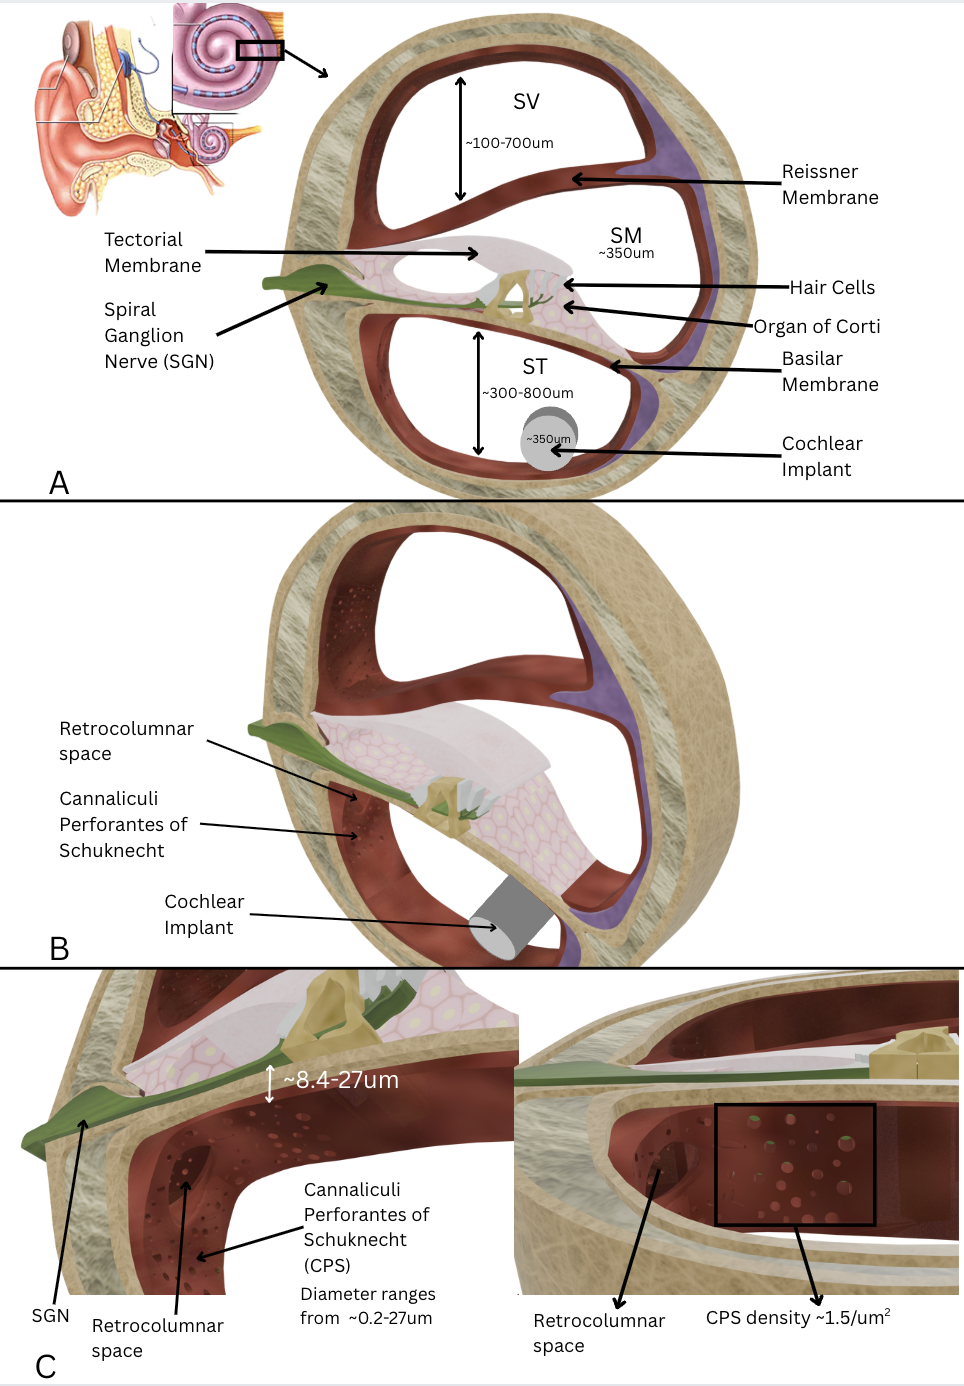
\includegraphics[width=0.8\textwidth]{Figure/3DAnatomyPanel.png}
  \caption{TBW}
  \label{fig:cochlea_overview}
\end{figure}
%%%%%%%%%%%%%%%%%%%%%%%%%%%%%
\subsection{Cochlear scalae in brief}  
The bony labyrinth encloses two perilymph‑filled channels, the \emph{scala vestibuli} and \emph{scala tympani}, which wind around the modiolus and communicate at the helicotrema. Sandwiched between them, the endolymphatic \emph{scala media} houses the organ of Corti on the basilar membrane.  Conventional cochlear implants occupy the scala tympani, placing their contacts within millimeters---but rarely microns---of spiral ganglion neurons (SGNs) embedded in Rosenthal’s canal. Importantly, typical electrode-to-SGN distances are around 0.5–1 mm for modiolus-hugging arrays and up to $\sim1.5-2 mm$ for lateral wall placements \cite{Davis2016}. Even in the best-case scenario, a gap on the order of $10^{2}-10^{3} \mu m$ remains between the electrode and neuron. This physical separation has practical implications: it necessitates current spread through perilymph and bone to reach the neurons, and it underlies why closer electrode positioning (e.g. perimodiolar designs) can reduce stimulation thresholds \cite{Kawano1998}. Furthermore, the distance can vary along the cochlea---apical electrodes often achieve the smallest gaps $\approx0.5 mm$ or less) while mid-cochlear electrodes can be $\approx1 mm$ or more away \cite{Long2014}. These quantitative insights, drawn from human studies, validate that CIs interface with the auditory nerve across a millimeter-scale gulf, rather than forming direct micron-level contact with the neurons. Finally, any natural pores linking the scala tympani to the modiolus are therefore potential highways for drugs, trophic factors, or neurites seeking the electrode array in the scala tympani.


\subsection{Scala Tympani Dimensions and Cochlear Implant feasibility}
\subsubsection{Scala Tympani Anatomy in Humans}
\paragraph{Human[Homo Sapiens]}
:  As briefly mentioned in a previous section, the human scala tympani is a large perilymph-filled canal that narrows from base to apex. Near the basal turn (around the round window region), the ST cross-section is ovoid with a typical vertical height of ~1.2–1.4 mm and width slightly larger \cite{fujiwara2023morphometric}. This corresponds to a cross-sectional area of roughly 2.3 mm² at the base (0°), which then diminishes to about 1.3–1.4 mm² by 180° (half a turn) into the cochlea \cite{fujiwara2023morphometric}. Beyond the basal turn (~360°), the ST lumen becomes more of a flattened triangle in cross-section as it enters the middle and apical turns. The height drops below 1 mm in the upper turns, and the area continues tapering (often $<$ 1 mm² near the apex). Thus, the basal ST can accommodate larger diameters, whereas the apical region is very small and slit-like. Notably, the ST width is consistently greater than its height at any given point \cite{hatsushika1990dimensions}, reflecting the elongated shape of the duct. The human cochlea is ~35–36 mm in uncoiled length (2.5–2.7 turns) and the total ST volume is about 29 $\mu$L \cite{Liu2023FEA}.

\subsection{Canaliculi Perforantes of Schuknecht (CPS)}  
Schuknecht’s original temporal‑bone study (1959) revealed hundreds of microscopic channels piercing the osseous spiral lamina (OSL) from the scala tympani toward the modiolus \cite{schuknecht1959}.  Later histology and scanning‑electron microscopy confirmed that these \textit{canaliculi perforantes} concentrate along the modiolar plate, especially in the basal and middle turns \cite{Schuknecht1963,lim1970,sando1971,masuda1971,tanaka1973}. The CPS are predominantly located on the scala tympani surface of the OSL, in the lower (inferior) bony lamina that underlies the basilar membrane. They are especially numerous in the modiolar (medial) region of the OSL, adjacent to the modiolus where the SGNs are housed \cite{shepherd2004}. Human CPS lumina were measured from 0.2 to 23 $\mu$ m against an OSL thickness that tapers from 26.8 $\mu$ m basally to 8.4 $\mu$ m apically \cite{shepherd2004}.  These dimensions overlap both the caliber of regenerating SGN neurites and the 10--30 $\mu$ m diffusion length of neurotrophins such as NT‑3 or BDNF in perilymph, making each pore a matched conduit for axonal ingress and trophic support.

\subsection{Other modiolar communication routes}  
\begin{enumerate}
\item Trabecular Meshwork: Rask‑Andersen and colleagues identified additional “trabecular meshwork” apertures—up to 100 $\mu$m in the scala vestibuli and 40 $\mu$ m in the scala tympani—plus fenestrations along perivascular and perineural sheaths \cite{raskandersen2006}.  Together with the CPS, they form a porous continuum that contradicts the notion of an impervious modiolar wall, permitting pressure equilibration and macromolecular traffic between perilymph and the SGN somata \cite{raskandersen2006, shepherd2004}.

\item Larger Modiolar Vascular Outlets: In addition, they identified "larger modiolar vascular outlets" as larger openings (up to $\sim$100 $\mu$m) adjacent to the anterior and posterior spiral modiolar veins and arteries, whose function is to permit exchange between perilymph and perivascular spaces, contributing to perilymph homeostasis and potential drug delivery routes. Finally, "mesothelial cell–covered fenestrae" was defined as thin cellular sheets ($<$ 3 $\mu$m) lining the OSL and modiolar surface, interspersed with micropores (up to $\sim$ 40 $\mu$m) on both the scala tympani and scala vestibuli sides. The function of mesothelial cell-covered fenestrae is to provide semi-permeable lining over the bony channels, allowing diffusion of small and large molecules while maintaining fluid compartmentalization \cite{raskandersen2006, shepherd2004}.

\item Mesothelial Cell–Covered Fenestrae: Thin cellular sheets ($<$ 3 $\mu$m) lining the OSL and modiolar surface, interspersed with micropores (up to $\sim$40 $\mu$m) on both the scala tympani and scala vestibuli sides. Mesothelial cell–covered fenestrae allows for exchange between perilymph and perivascular spaces, contributing to perilymph homeostasis and potential drug delivery routes \cite{raskandersen2006, shepherd2004}.

\end{enumerate}

\begin{table}[ht]
\centering
\caption{Quantitative dimensions of perilymph–modiolar passage channels in the basal turn of the human cochlea}
\label{tab:channels_dimensions}
\begin{tabular}{lll}
\toprule
\textbf{Structure / Channel} & \textbf{Dimension (basal turn)} & \textbf{Source} \\
\midrule
Canaliculi Perforantes Schuknecht (CPS) & Mean diameter $5.2 \pm 4.9\ \mu$m (range 0.2--23.0 $\mu$m)       & \cite{ShepherdColreavy2004} \\
Osseous spiral lamina (OSL) thickness & $26.8 \pm 6.0\ \mu$m                                      & \cite{ShepherdColreavy2004} \\
Density of canaliculi (pores/$\mu$m²)   & $1.05 \pm 1.03$ pores/$\mu$m²                                  & \cite{ShepherdColreavy2004} \\
Mesothelial cell–sheet thickness    & $0.3$--$3\ \mu$m                                            & \cite{raskandersen2006} \\
Trabecular‐mesh “fenestrae” size    & Up to $\sim 40\ \mu$m (holes in modiolar wall)             & \cite{raskandersen2006} \\
Modiolar vascular outlets           & Pores up to $\sim 100\ \mu$m                               & \cite{raskandersen2006} \\
\bottomrule
\end{tabular}
\end{table}

\subsection{Functional Pathways and SGN Connectivity Through CPS}
The CPS form a network of microscopic pores through the OSL that directly links the fluid of the scala tympani with the perimodiolar spaces in Rosenthal’s canal \cite{raskandersen2006}. By puncturing the lower plate of the OSL---alongside gaps in its mesothelial lining---and opening into the retrocolumnar trabecular meshwork and perivascular channels of the modiolus, these tiny canals create a continuous perilymphatic pathway from the ST into the SGNs. As a result, the extracellular fluid bathing the SGN cell bodies is essentially the same perilymph that fills the scala tympani, permitting free interchange of ions, nutrients, signaling molecules, and even therapeutic agents or pathogens between these compartments.

Although the true nerve fiber bundles use larger foramina (habenula perforata and modiolar conduits) to enter and exit Rosenthal’s canal, the canaliculi perforantes run alongside and between those fiber routes, serving as perineural and perivascular fluid conduits. Glueckert et al. found nerve fibers in BDNF-treated animals that progressed into CPS. These fibers reveal a myelin layer close to the OSL and within the bony canaliculi but with extreme swelling when entering the scala typani \cite{glueckert2008}. Li et al. also observed SGN neurites projecting across the OSL wall into the ST through the CPS \cite{Li2017}. Similar observations have been reported by others \cite{Staecker1996, Leake2008, Leake2011, Wise2011}.  

\subsection{Distance Between Cochlear Implant Electrodes and Spiral Ganglion Neurons in Rosenthal’s Canal}
Conventional CI electrode arrays reside in the scala tympani and thus are separated from the SGNs in Rosenthal’s canal by the bony modiolus. Multiple anatomical and imaging studies confirm that across patients and electrode positions, the distance between an electrode contact and the SGNs in Rosenthal’s canal generally spans from a few hundred microns up to $\sim$1–2 mm. A detailed CT scan study of perimodiolar arrays reported a total range of $\sim$0.1 mm up to 1.8 mm in electrode-to-modiolus separation \cite{Long2014}. Histological section measurements estimate that in the human basal turn, a lateral-wall electrode may be roughly $\sim$2 mm away from the spiral ganglion (by radial distance). These data support the statement that CI contacts lie within millimeters—but rarely mere microns—of the SGNs\cite{Schmidbauer2023}.

The electrode-to-SGN distance is not uniform along the cochlea; it varies with the cochlear turn and electrode position. Overall, the closest electrode-neuron proximities are achieved in the apical cochlea, with mid-cochlea generally the farthest on average, though patient-specific anatomy causes considerable variability (overall 0.1--1.8 mm range in the cited study) \cite{Long2014}.

\subsection{The Electrode-Neuron Gap Does Matter}
Kawano et al. (1998) performed detailed histopathologic exams of five human cochleae with CIs and measured the distance between each electrode band and the center of Rosenthal’s canal \cite{Kawano1998}. They reported that these electrode-to-SGN distances were in the millimeter range, and importantly found a correlation between greater distance and higher electrical thresholds and comfort levels. In other words, electrodes that sat farther (several millimeters) from the SGNs required more current to evoke hearing, reinforcing that distance is a key factor. The same study noted that intracochlear fibrosis or new bone formation could increase the electrode-modiolus distance, sometimes pushing contacts farther than their design intends. Nadol and colleagues, in histopathologic surveys, likewise estimated distances on the order of 0.5–2 mm and observed that any translocation of an array out of scala tympani (or trauma to the modiolus) can reduce SGN counts, further emphasizing that the electrode-neuron gap matters \cite{nadol1990,Nadol1989}. Computational models and anatomic maps further illustrate these distances. For example, a recent finite-element model by Sriperumbudur et al. (2024) examined electrical stimulation with a perimodiolar CI and assumed a ~0.3 mm gap between the electrode and modiolus as a typical design. This value (300 $\mu$ m) was chosen to reflect a snug perimodiolar placement, yet it still highlights that even in simulation the contacts are not assumed to be touching the neurons (a 0.3 mm gap leaves space for the bony wall and perilymph) \cite{Sriperumbudur2024}. 

\subsection{Surgical implications for biohybrid CIs}  
Because CPS density peaks in the basal OSL, traumatic insertion or aggressive drilling in this region risks sealing the very pathways that a biohybrid implant aims to exploit \cite{shepherd2004}.  Conversely, electrodes engineered with microfluidic ports or neurotrophin‑releasing sleeves could harness these pores to establish steep radial gradients that attract transplanted or residual neurites toward the contacts.  Designing arrays that spare, rather than violate, the CPS therefore becomes as important as thread depth, pitch, or perimodiolar curl.  Leveraging these natural conduits should reduce reliance on bulk diffusion, localize therapy to the modiolus, and ultimately tighten the electrode–neuron interface—a prerequisite for the stem‑cell and material strategies developed in the following sections. Future biohybrid implants are expected to incorporate microfluidic drug delivery (e.g., convection‑enhanced or electrically driven release) to steer regeneration locally within the cochlea \cite{Carnicer-Lombarte:2025aa}.

